
\section{Overview}
The overall workflow of the project is illustrated in Figure~\ref{fig:framework}.

\begin{figure}[!h]
    \centering
    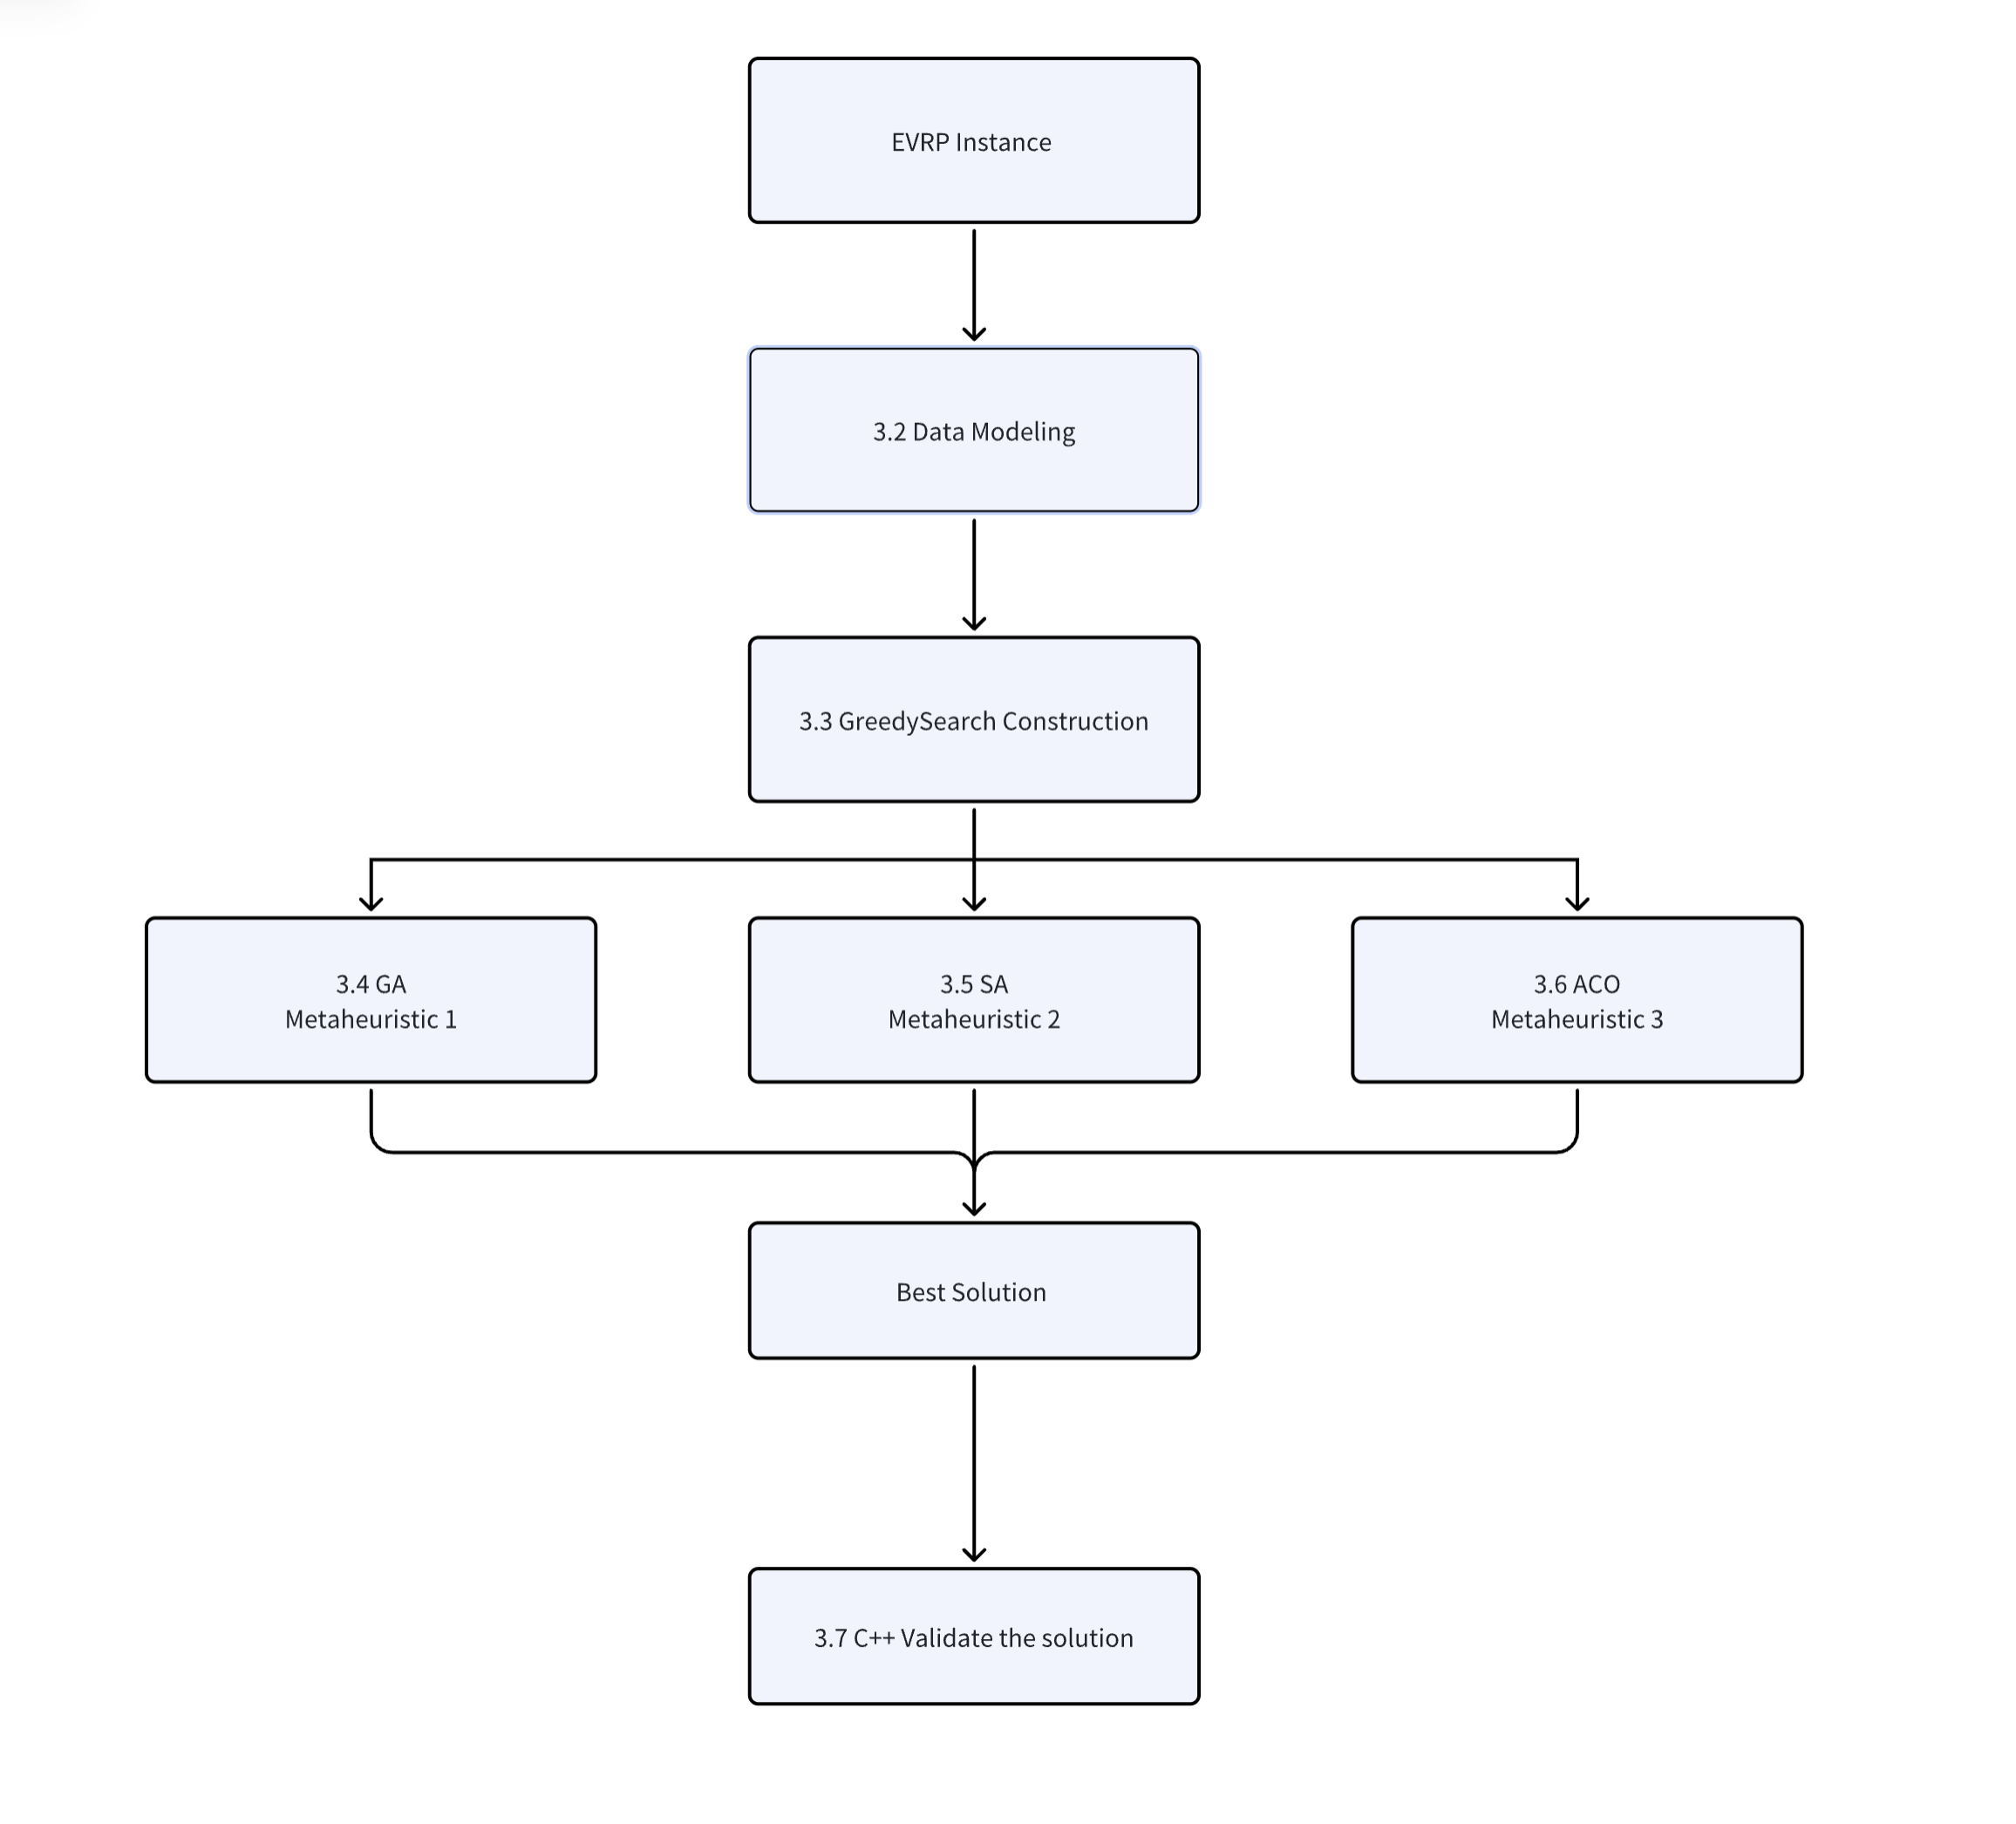
\includegraphics[width=0.7\linewidth]{image/3/framework.png}
    \caption{Overall framework of the proposed solution.}
    \label{fig:framework}
\end{figure}

The process begins with the selection of an EVRP (Electric Vehicle Routing Problem) instance.  
In Section~\ref{sec:data_modeling}, the data is modeled to represent the problem environment, including customer locations, charging stations, and vehicle constraints.  
Next, in Section~\ref{sec:greedy_search}, an initial feasible solution is constructed using a Greedy Search strategy to provide a starting point for further optimization.  
Subsequently, three different metaheuristic approaches are applied separately: Genetic Algorithm in Section~\ref{sec:ga}, Simulated Annealing in Section~\ref{sec:sa}, and Ant Colony Optimization in Section~\ref{sec:aco}.  
Each method searches for high-quality solutions independently.  
Afterward, the best solution among the three is selected.  
Finally, in Section~\ref{sec:cpp_validation}, a C++ program is used to validate the correctness and feasibility of the obtained solution.




\section{Problem Formulation}

The Electric Vehicle Routing Problem (EVRP) considered in this project is formulated on a complete undirected graph \( G = (V, E) \), where \( V \) denotes the set of all nodes and \( E \) represents the set of edges connecting pairs of nodes. The node set \( V \) is partitioned into three disjoint subsets: the depot \( D \), the set of customers \( C \), and the set of charging stations \( S \), satisfying:
\[
V = D \cup C \cup S
\]

Each edge \( (i, j) \in E \) is associated with a non-negative Euclidean distance \( d_{ij} \) and an energy consumption \( e_{ij} = h \times d_{ij} \), where \( h > 0 \) denotes the energy consumption rate per unit distance.

A homogeneous fleet of vehicles is available, each characterized by:
\begin{itemize}
    \item A maximum load capacity \( C \) for carrying customer demands.
    \item A maximum battery capacity \( Q \) limiting travel between recharges.
\end{itemize}

Each customer node \( i \in C \) has a demand \( q_i \geq 0 \). Charging stations \( S \) and the depot \( D \) offer opportunities for full battery replenishment.

The goal of EVRP is to construct a set of routes, each starting and ending at the depot, while minimizing total travel distance and satisfying the following constraints:

\begin{itemize}
    \item \textbf{Service constraint}: Each customer must be visited exactly once by a vehicle.
    \item \textbf{Capacity constraint}: The total demand served in a route must not exceed vehicle capacity \( C \).
    \item \textbf{Energy constraint}: The cumulative energy consumed between consecutive recharge opportunities must not exceed battery capacity \( Q \).
\end{itemize}

Formally, the objective is:
\[
\min \sum_{k \in K} \sum_{(i, j) \in r_k} d_{ij}
\]
where \( r_k \) is the sequence of nodes visited by vehicle \( k \).

This formulation captures the combined logistical (load) and energy (battery) constraints, making EVRP a complex and realistic extension of the classical Vehicle Routing Problem (VRP).

\bigskip

\section{Data Representation and Problem Setup}
\label{sec:data_modeling}

To enable computational implementation of the above formulation, the EVRP instance is structured into a set of data representations as follows.

Each node \( i \in V \) is modeled with attributes:
\begin{itemize}
    \item Unique identifier \( \text{id}_i \).
    \item Coordinates \( (x_i, y_i) \) in two-dimensional Euclidean space.
    \item Node type: customer, charging station, or depot.
    \item Demand \( q_i \geq 0 \) (positive for customers, zero otherwise).
\end{itemize}

The Euclidean distance between nodes \( i \) and \( j \) is calculated as:
\[
d_{ij} = \sqrt{(x_i - x_j)^2 + (y_i - y_j)^2}
\]
and the corresponding energy consumption is:
\[
e_{ij} = h \times d_{ij}
\]
with \( h \) specified for each problem instance.

The full problem setup includes:
\begin{itemize}
    \item Customer set \( C \) and their demands.
    \item Charging station set \( S \).
    \item Depot node \( D \).
    \item Distance matrix \( \{ d_{ij} \} \) and energy matrix \( \{ e_{ij} \} \).
    \item Vehicle parameters: capacity \( C \) and battery limit \( Q \).
\end{itemize}

To accelerate metaheuristic search procedures, a precomputed nearest-neighbor list \( \mathcal{N}(i) \) for each node is optionally constructed, sorted by ascending distance.

\bigskip
\noindent\textbf{Solution Validation}

Any proposed solution must satisfy:
\begin{itemize}
    \item Each customer is visited exactly once.
    \item No route exceeds the vehicle's load capacity.
    \item No route exceeds the battery capacity between recharge points.
\end{itemize}
Feasibility checks are systematically enforced to ensure all evaluated solutions are valid under the problem constraints.


\section{Initial Solution Construction: Greedy Search Algorithm}
\label{sec:greedy_search}

To construct an initial feasible solution for the Electric Vehicle Routing Problem (EVRP), a multi-stage greedy heuristic is employed.  
The method progressively builds capacity-aware and energy-feasible routes by clustering customers, inserting depots and charging stations when necessary, and applying local optimization. The procedure consists of the following stages:

\subsection{Problem Setup}

The \texttt{GreedySearch} algorithm is initialized with a \texttt{Problem} instance, which provides access to customer nodes, charging stations, the depot, and global parameters such as vehicle load capacity \( C \) and battery capacity \( Q \).

To accelerate the search process, two nearest-neighbor matrices are precomputed:
\begin{itemize}
    \item \textbf{Customer-Customer Nearest Neighbor Matrix}: Facilitates fast clustering of customers.
    \item \textbf{Node-Station Nearest Neighbor Matrix}: Enables rapid identification of charging stations for energy management.
\end{itemize}

\subsection{Customer Clustering}

An initial set of tours is constructed by greedily clustering customers based on spatial proximity and vehicle load constraints:
\begin{itemize}
    \item Customers are randomly shuffled to introduce initialization diversity.
    \item A center customer is selected to seed each tour, with nearby customers added sequentially without exceeding capacity \( C \).
    \item If the maximum number of vehicles is reached, any remaining unassigned customers are appended to the last tour.
    \item Empty tours are padded if necessary to match the fleet size.
\end{itemize}

\subsection{Capacity Balancing}

To improve fleet utilization, customers from overloaded tours are reallocated to underloaded ones whenever possible, prioritizing proximity and load balancing.

\subsection{Local Search Optimization (2-Opt)}

Each tour undergoes local refinement via the classical 2-opt heuristic:
\begin{itemize}
    \item Non-adjacent edges are iteratively swapped to reduce total travel distance.
    \item Optimization continues until no further improvements are found.
\end{itemize}

\subsection{Depot Insertion}

Depot nodes are inserted dynamically to maintain vehicle load feasibility:
\begin{itemize}
    \item When cumulative load threatens to exceed \( C \), a depot is inserted to allow reloading.
    \item Depot positions are greedily optimized to minimize additional travel distance.
\end{itemize}

\subsection{Charging Station Insertion and Optimization}

Energy constraints are enforced by strategically inserting charging stations:
\begin{itemize}
    \item When insufficient energy remains to reach the next node, the nearest feasible charging station is inserted.
    \item Greedy replacements are attempted to substitute inefficient charging stations with better alternatives without violating feasibility.
\end{itemize}

\subsection{Solution Finalization}

The finalized tours are encapsulated into a \texttt{Solution} object, ensuring compliance with both load and energy constraints.  
This initial solution provides a high-quality, feasible starting point for subsequent metaheuristic optimization stages.

\bigskip
This multi-stage greedy construction strategy ensures that the initial solution is not only feasible but also sufficiently optimized to accelerate convergence of higher-level algorithms such as GA, SA, and ACO.





\section{Metaheuristic Optimization: Greedy-Search Genetic Algorithm}
\label{sec:ga}
\begin{figure}[!h]
    \centering
    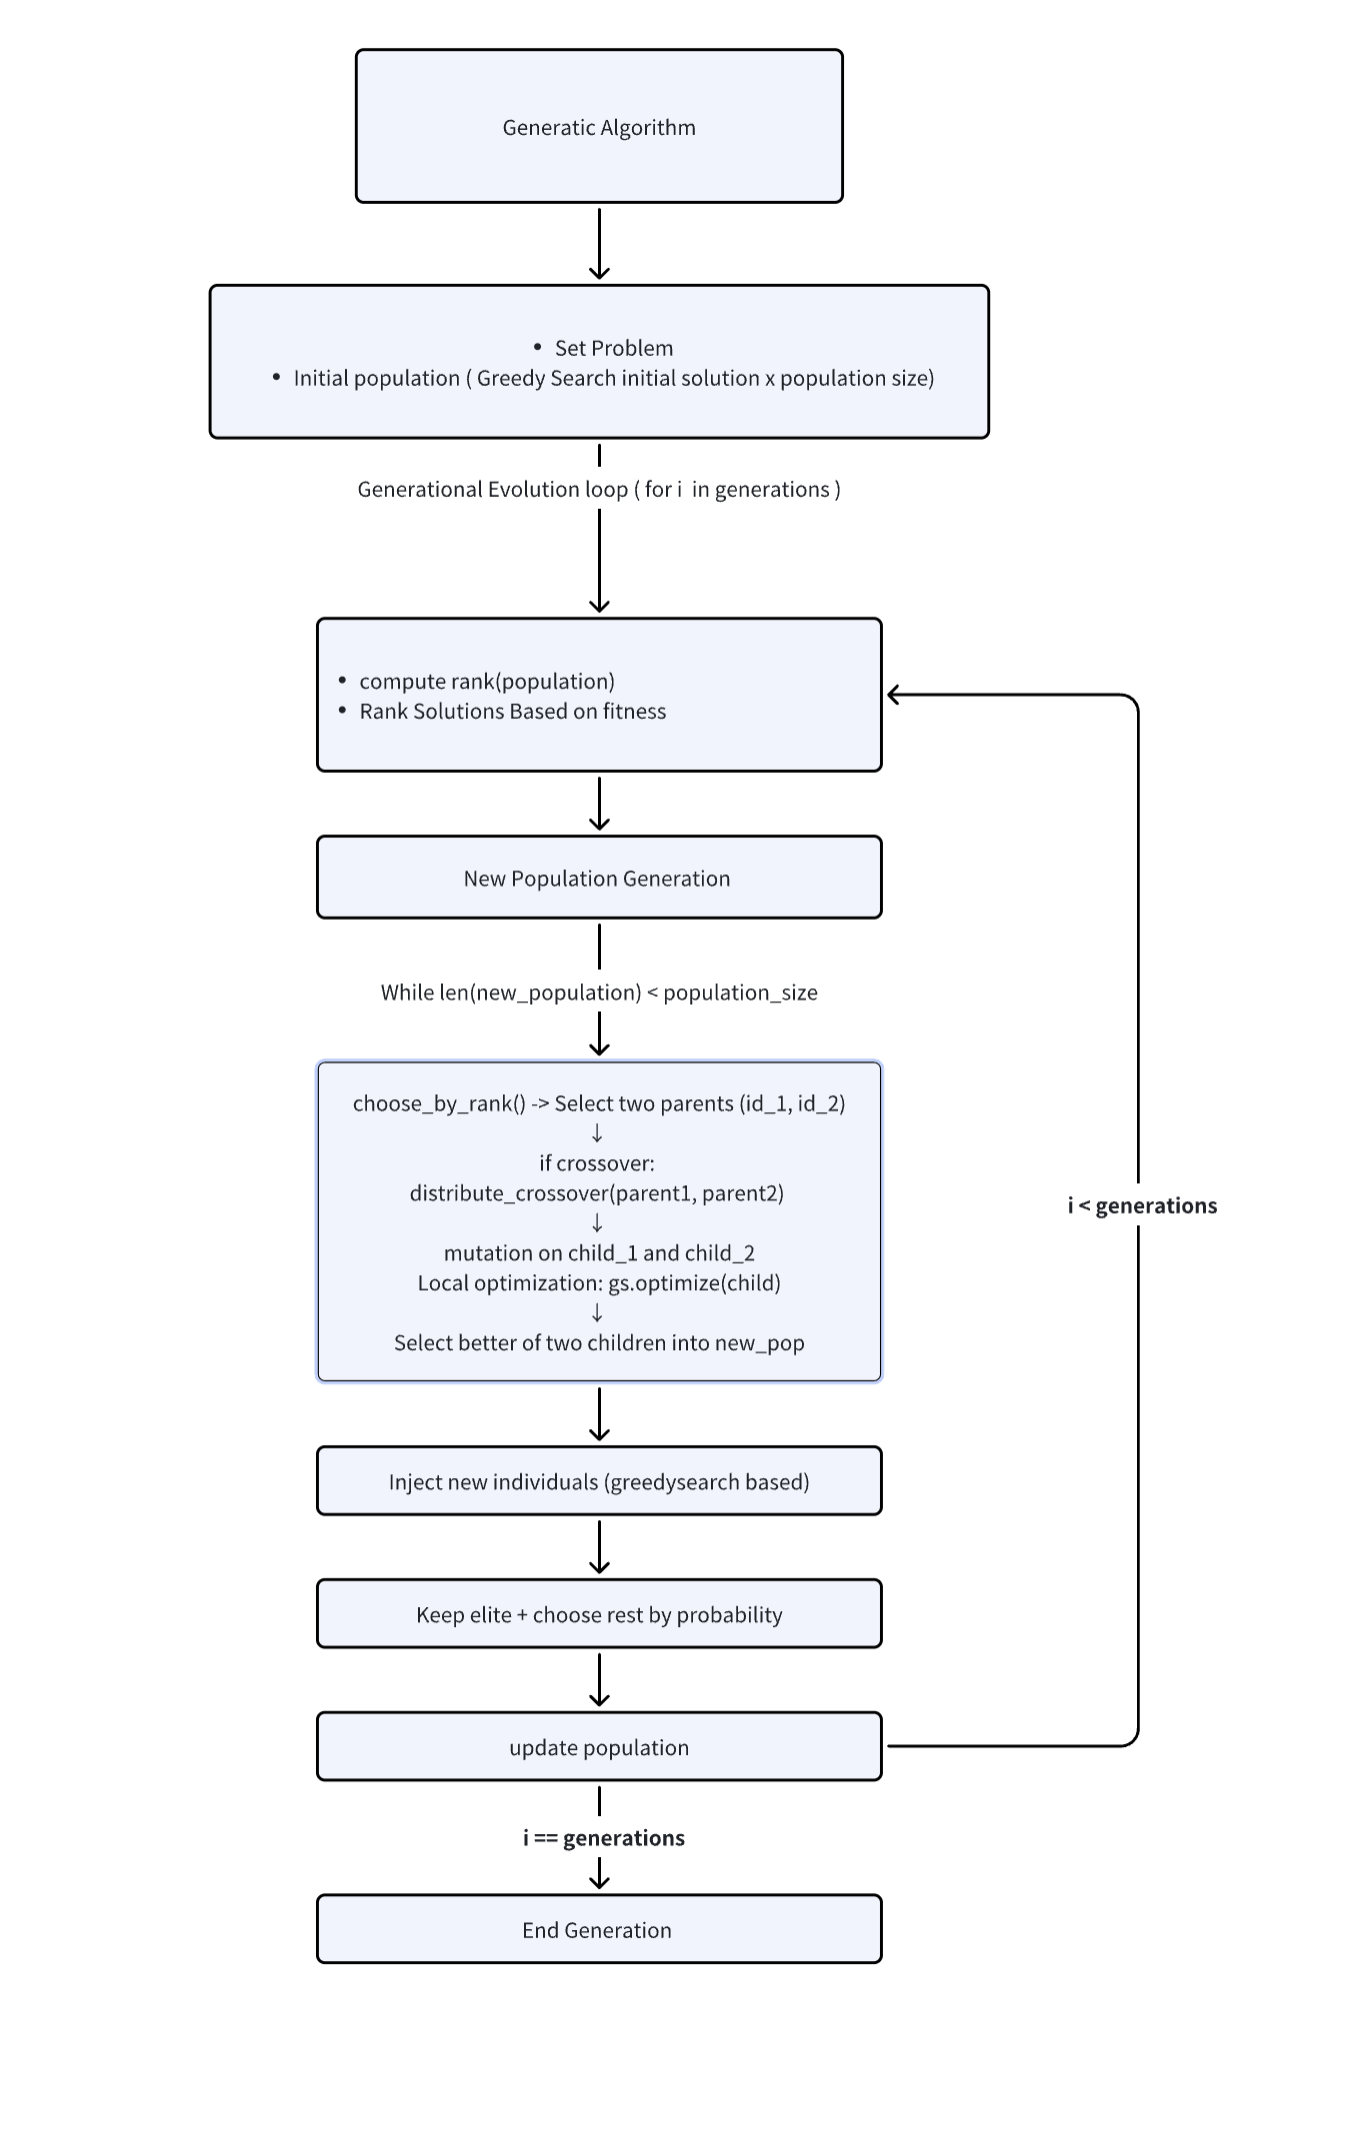
\includegraphics[width=0.7\linewidth]{image/3/gaflow.png}
    \caption{GA's flow chart}
    \label{fig:gaflow}
\end{figure}
Furthermore, the GA is developed based on this work~\cite{hien2023greedy}(Fig.~\ref{fig:gaflow}). This method integrates evolutionary exploration with domain-specific greedy optimization to achieve a balance between diversification and intensification.  
The optimization process is organized into the following stages:

First, the initial population is generated by applying greedy clustering and local search to randomized customer assignments, ensuring both feasibility and diversity.  
An elitist selection strategy is employed, preserving a fixed proportion of top-performing individuals while sampling the remainder via fitness-proportional probabilities to promote exploration.

Offspring are created through a distribute crossover operator, reallocating customer subsets between two parents while preserving route feasibility.  
Mutation is applied probabilistically to offspring, dynamically selecting among heavy mutation (HMM), heavy swap mutation (HSM), and random swap mutation operators according to a cosine-decay schedule, gradually shifting focus from exploration to exploitation.

Each offspring undergoes greedy local repair to correct constraint violations and improve solution quality.  
To mitigate premature convergence, a portion of each generation is periodically refreshed by injecting new greedy-optimized individuals.

The evolutionary process is iterated for a fixed number of generations, continuously updating the best solution found and dynamically adjusting operator selection intensity according to progress.

\section{Metaheuristic Optimization: Simulated Annealing}
\label{sec:sa}
\begin{figure}[!h]
    \centering
    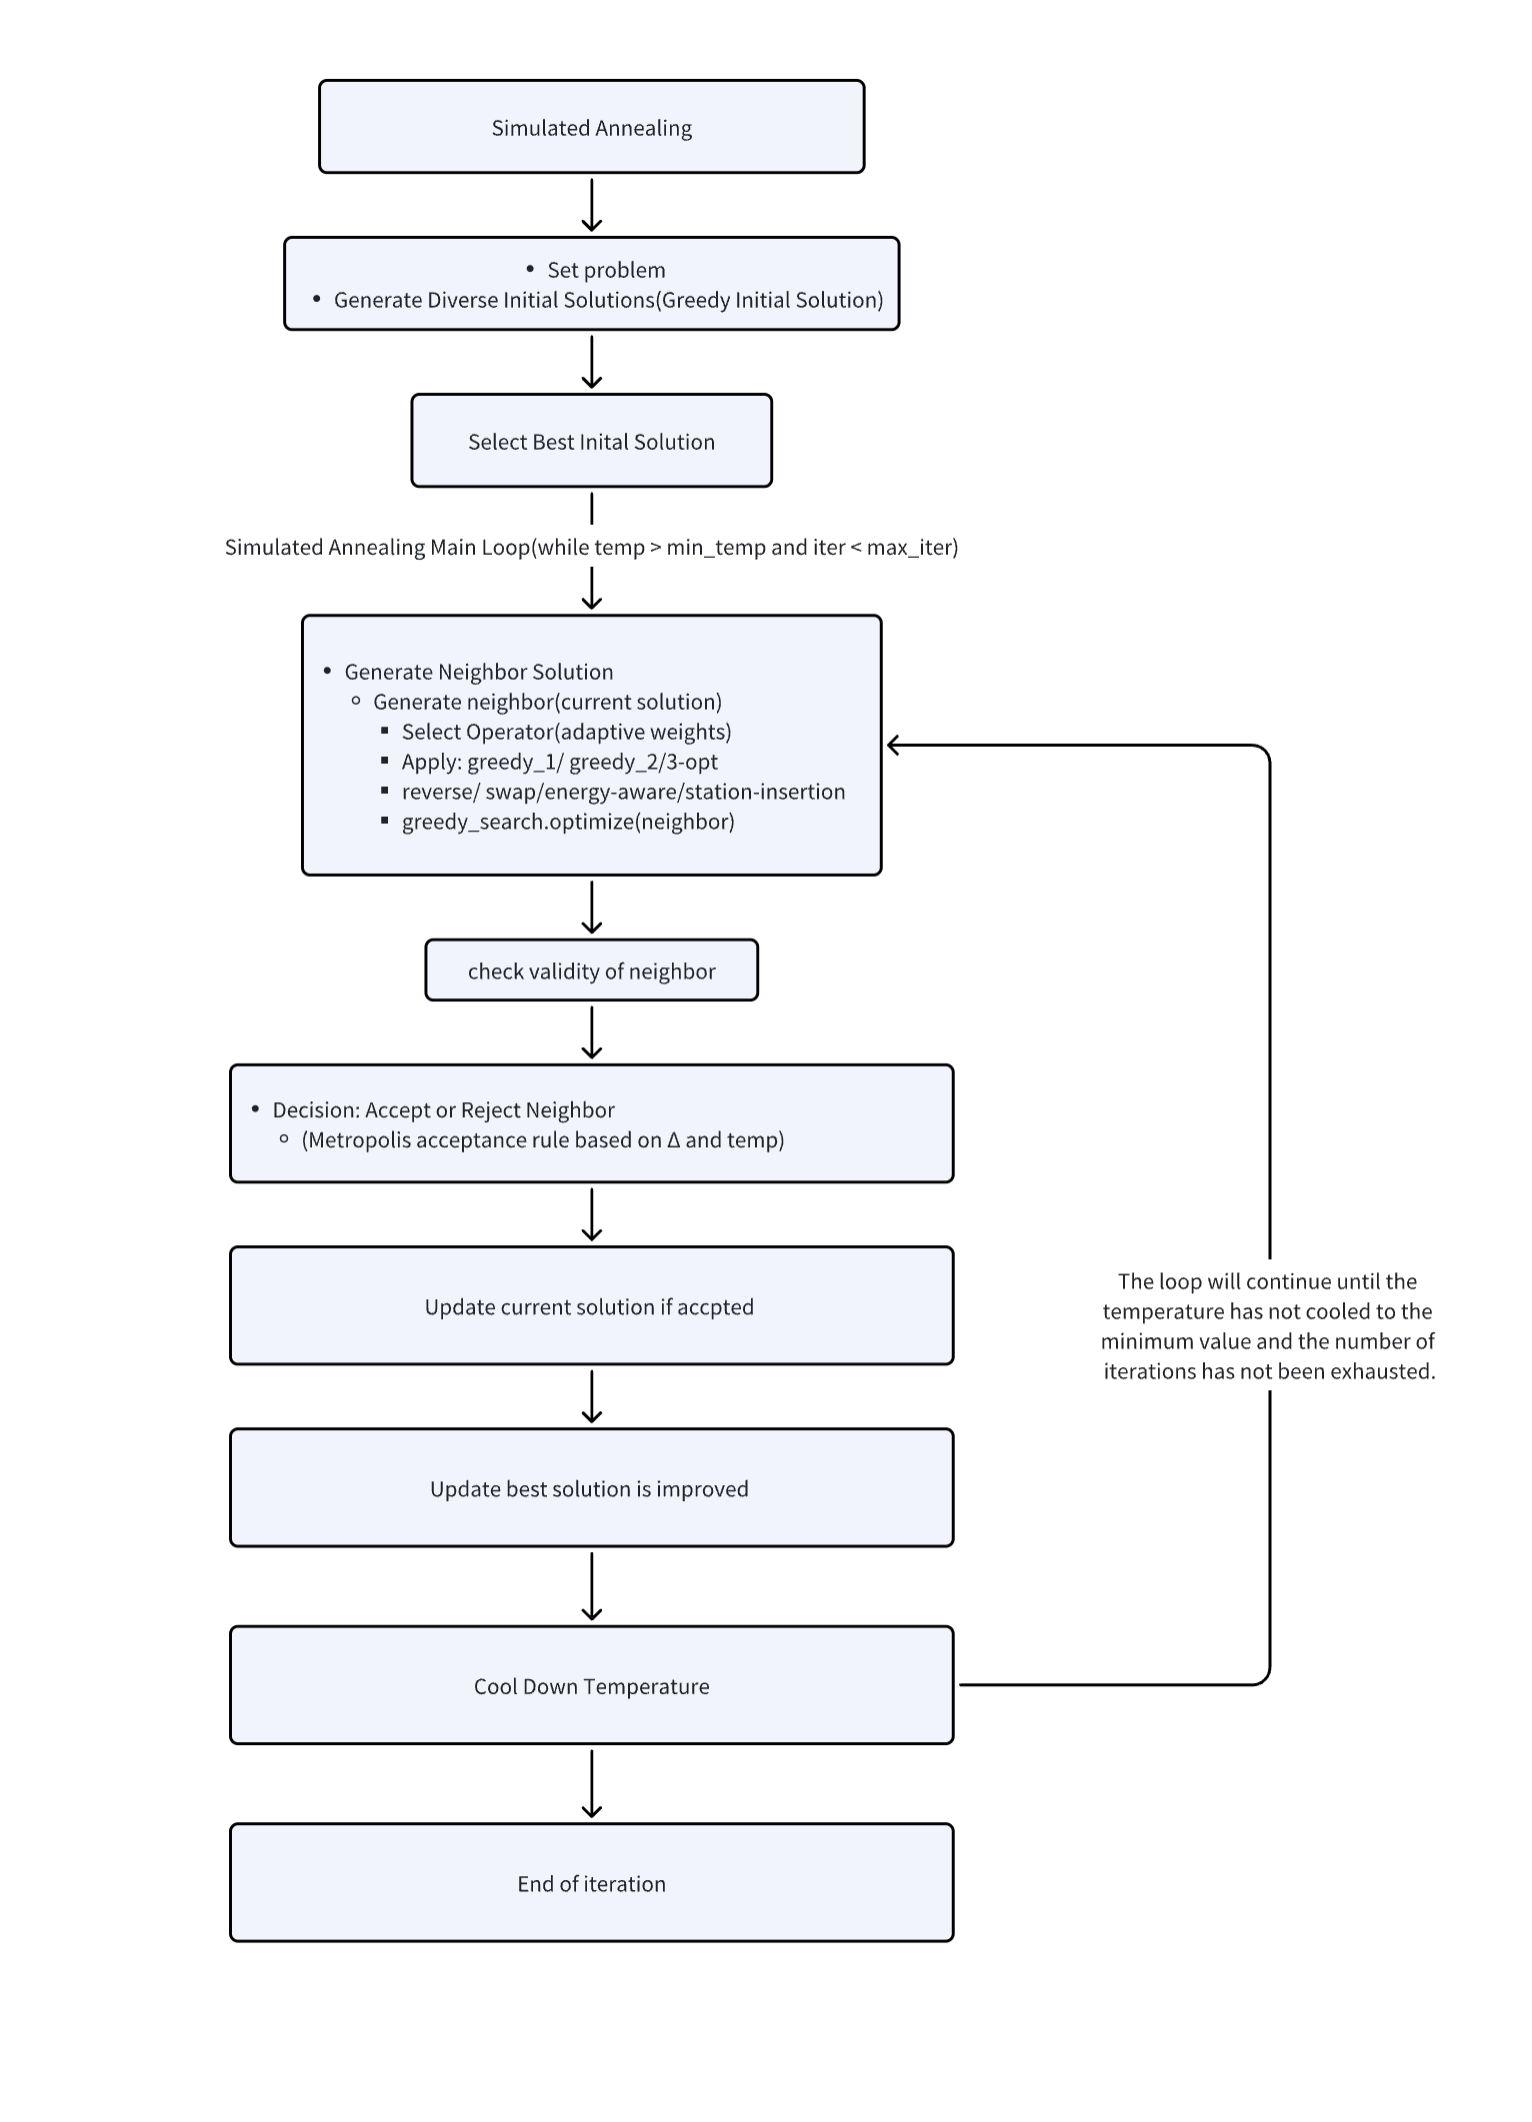
\includegraphics[width=0.7\linewidth]{image/3/saflow.png}
    \caption{Simulated Annealing}
    \label{fig:saflow}
\end{figure}
The Simulated Annealing method is shown as Fig.~\ref{fig:saflow}. The method integrates adaptive temperature control, diversified neighborhood operators, energy-aware mutation strategies, and intensive local search to effectively balance exploration and exploitation.  
The optimization process is structured as follows:

The search is initialized with a diverse set of feasible solutions generated through greedy construction, random perturbation, and energy-aware mutations. The best among them is selected as the starting point.

During the annealing process, neighbor solutions are generated adaptively using multiple operators, including customer exchanges, 2-opt, 3-opt, segment reversals, and energy-focused mutations.  
Operator selection is guided by dynamic success tracking, favoring effective moves while maintaining diversity.

New solutions are accepted according to the Metropolis criterion, with acceptance probability decreasing under an adaptive cooling schedule that adjusts based on search progress and stagnation.  
Infeasible neighbor solutions are repaired or replaced by fresh greedy-optimized candidates through a multi-stage repair strategy.

To prevent search stagnation, reheating and strong diversification strategies are triggered when no improvement is observed over predefined iterations, involving customer shuffling and tour restructuring followed by greedy repair.

Finally, an iterated local search phase combining random perturbations and intensive local refinements across multiple neighborhoods is applied to further improve the best solution found.



\section{Metaheuristic Optimization: Ant Colony Optimization}
\label{sec:aco}
\begin{figure}[!h]
    \centering
    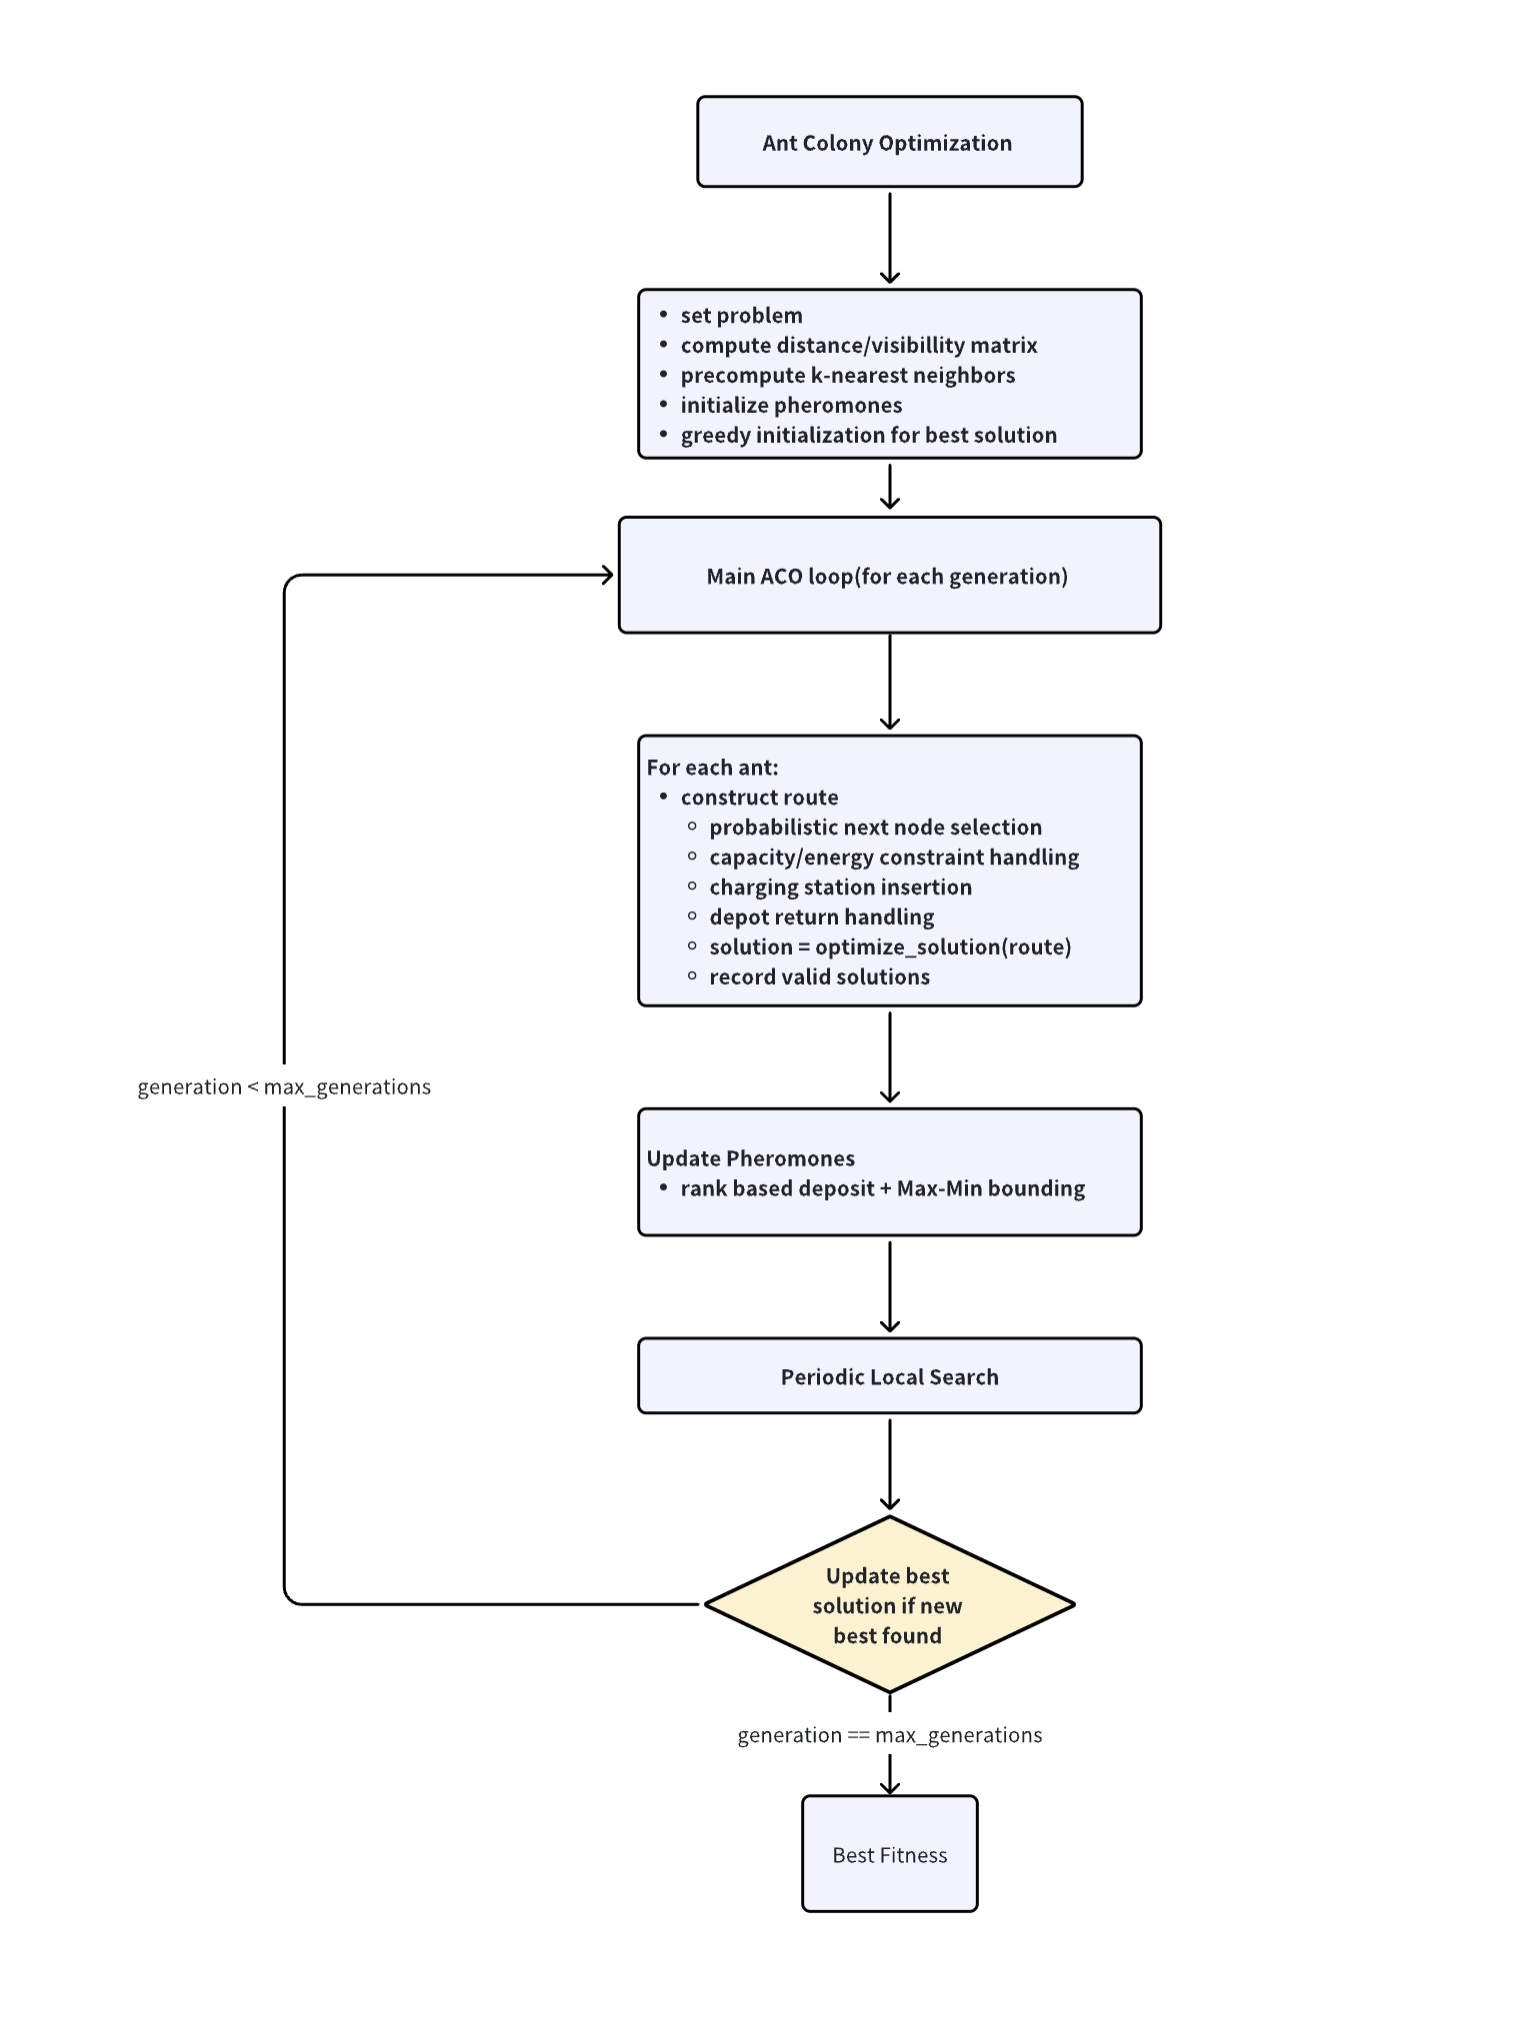
\includegraphics[width=0.7\linewidth]{image/3/acoflow.png}
    \caption{Ant Colony Optimization}
    \label{fig:acoflow}
\end{figure}
Our Ant Colony Optimization method is described in fig.~\ref{fig:acoflow}
The method combines probabilistic construction, adaptive pheromone management, local refinement strategies, and dynamic perturbation mechanisms to balance exploration and exploitation effectively.  
The optimization process is structured as follows:

Each ant constructs a feasible solution by probabilistically selecting the next node based on pheromone strength and heuristic visibility, considering energy and capacity constraints.  
To guide efficient construction, only a limited set of $K$ nearest neighbors is evaluated for each decision.

Constructed solutions are refined through multiple local search strategies, including greedy optimization, customer exchange within tours, load redistribution across tours, and intensive 2-opt and 3-opt operators.  
These refinements ensure that solutions not only satisfy all constraints but also minimize total route length.

After all ants complete their routes, pheromone trails are updated based on solution quality, applying a rank-based elitist reinforcement strategy combined with a Max-Min pheromone bounding rule to stabilize search behavior.  
The best global solution receives additional pheromone reinforcement across generations.

To maintain search diversity and avoid premature convergence, a pheromone perturbation mechanism is applied periodically, blending pheromone values toward their mean based on the degree of search stagnation.

Throughout the process, stagnation detection and early stopping criteria are incorporated, triggering intensified diversification and pheromone perturbation if improvement stalls over consecutive generations.  
Final solutions undergo an intensive local search phase to ensure high solution quality before termination.

\section{Solution Validation Using C++}
\label{sec:cpp_validation}
To ensure the correctness of all generated solutions, a dedicated C++ validation tool was implemented.  
This tool verifies that each solution starts and ends at the depot, visits all customers exactly once, respects vehicle capacity and battery energy constraints throughout the route, and properly handles recharging at charging stations or the depot.  
The validator also calculates the total route length and reports the optimality gap if a known optimum is available.  
By performing thorough consistency and feasibility checks at the solution level, this C++ validator guarantees the accuracy and reliability of the experimental results.
